\chapter{Directed graphs}

In this chapter, we focus on two classes of directed graphs:

\begin{itemize}
\item \key{Acyclic graphs}:
There are no cycles in the graph,
so there is no path from any node to itself\footnote{Directed acyclic
graphs are sometimes called DAGs.}.
\item \key{Successor graphs}:
The outdegree of each node is 1,
so each node has a unique successor.
\end{itemize}
It turns out that in both cases,
we can design efficient algorithms that are based
on the special properties of the graphs.

\section{Topological sorting}

\index{topological sorting}
\index{cycle}

A \key{topological sort} is a ordering
of the nodes of a directed graph
such that if there is a path from node $a$ to node $b$,
then node $a$ appears before node $b$ in the ordering.
For example, for the graph
\begin{center}
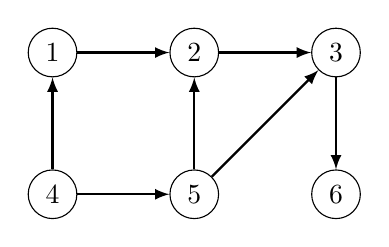
\begin{tikzpicture}[scale=0.9]
\node[draw, circle] (1) at (1,5) {$1$};
\node[draw, circle] (2) at (3,5) {$2$};
\node[draw, circle] (3) at (5,5) {$3$};
\node[draw, circle] (4) at (1,3) {$4$};
\node[draw, circle] (5) at (3,3) {$5$};
\node[draw, circle] (6) at (5,3) {$6$};

\path[draw,thick,->,>=latex] (1) -- (2);
\path[draw,thick,->,>=latex] (2) -- (3);
\path[draw,thick,->,>=latex] (4) -- (1);
\path[draw,thick,->,>=latex] (4) -- (5);
\path[draw,thick,->,>=latex] (5) -- (2);
\path[draw,thick,->,>=latex] (5) -- (3);
\path[draw,thick,->,>=latex] (3) -- (6);
\end{tikzpicture}
\end{center}
a possible topological sort is
$[4,1,5,2,3,6]$:
\begin{center}
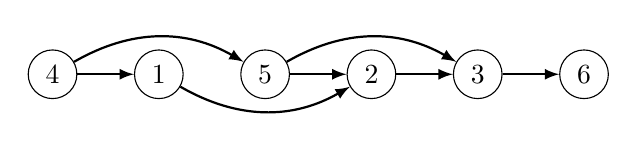
\begin{tikzpicture}[scale=0.9]
\node[draw, circle] (1) at (-6,0) {$1$};
\node[draw, circle] (2) at (-3,0) {$2$};
\node[draw, circle] (3) at (-1.5,0) {$3$};
\node[draw, circle] (4) at (-7.5,0) {$4$};
\node[draw, circle] (5) at (-4.5,0) {$5$};
\node[draw, circle] (6) at (-0,0) {$6$};

\path[draw,thick,->,>=latex] (1) edge [bend right=30] (2);
\path[draw,thick,->,>=latex] (2) -- (3);
\path[draw,thick,->,>=latex] (4) -- (1);
\path[draw,thick,->,>=latex] (4) edge [bend left=30] (5);
\path[draw,thick,->,>=latex] (5) -- (2);
\path[draw,thick,->,>=latex] (5) edge [bend left=30]  (3);
\path[draw,thick,->,>=latex] (3) -- (6);
\end{tikzpicture}
\end{center}

An acyclic graph always has a topological sort.
However, if the graph contains a cycle,
it is not possible to form a topological sort,
because no node in the cycle can appear
before the other nodes in the cycle.
It turns out that depth-first search can be used
to both check if a directed graph contains a cycle
and, if it does not contain a cycle, to construct a topological sort.

\subsubsection{Algorithm}

The idea is to go through the nodes of the graph
and always begin a depth-first search at the current node
if it has not been processed yet.
During the searches, the nodes have three possible states:

\begin{itemize}
\item state 0: the node has not been processed (white)
\item state 1: the node is under processing (light gray)
\item state 2: the node has been processed (dark gray)
\end{itemize}

Initially, the state of each node is 0.
When a search reaches a node for the first time,
its state becomes 1.
Finally, after all successors of the node have
been processed, its state becomes 2.

If the graph contains a cycle, we will find out this
during the search, because sooner or later
we will arrive at a node whose state is 1.
In this case, it is not possible to construct a topological sort.

If the graph does not contain a cycle, we can construct
a topological sort by 
adding each node to a list when the state of the node becomes 2.
This list in reverse order is a topological sort.

\subsubsection{Example 1}

In the example graph, the search first proceeds
from node 1 to node 6:

\begin{center}
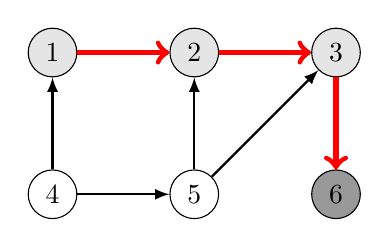
\begin{tikzpicture}[scale=0.9]
\node[draw, circle,fill=gray!20] (1) at (1,5) {$1$};
\node[draw, circle,fill=gray!20] (2) at (3,5) {$2$};
\node[draw, circle,fill=gray!20] (3) at (5,5) {$3$};
\node[draw, circle] (4) at (1,3) {$4$};
\node[draw, circle] (5) at (3,3) {$5$};
\node[draw, circle,fill=gray!80] (6) at (5,3) {$6$};

\path[draw,thick,->,>=latex] (4) -- (1);
\path[draw,thick,->,>=latex] (4) -- (5);
\path[draw,thick,->,>=latex] (5) -- (2);
\path[draw,thick,->,>=latex] (5) -- (3);
%\path[draw,thick,->,>=latex] (3) -- (6);

\path[draw=red,thick,->,line width=2pt] (1) -- (2);
\path[draw=red,thick,->,line width=2pt] (2) -- (3);
\path[draw=red,thick,->,line width=2pt] (3) -- (6);
\end{tikzpicture}
\end{center}

Now node 6 has been processed, so it is added to the list.
After this, also nodes 3, 2 and 1 are added to the list:

\begin{center}
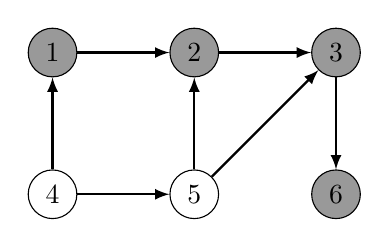
\begin{tikzpicture}[scale=0.9]
\node[draw, circle,fill=gray!80] (1) at (1,5) {$1$};
\node[draw, circle,fill=gray!80] (2) at (3,5) {$2$};
\node[draw, circle,fill=gray!80] (3) at (5,5) {$3$};
\node[draw, circle] (4) at (1,3) {$4$};
\node[draw, circle] (5) at (3,3) {$5$};
\node[draw, circle,fill=gray!80] (6) at (5,3) {$6$};

\path[draw,thick,->,>=latex] (1) -- (2);
\path[draw,thick,->,>=latex] (2) -- (3);
\path[draw,thick,->,>=latex] (4) -- (1);
\path[draw,thick,->,>=latex] (4) -- (5);
\path[draw,thick,->,>=latex] (5) -- (2);
\path[draw,thick,->,>=latex] (5) -- (3);
\path[draw,thick,->,>=latex] (3) -- (6);
\end{tikzpicture}
\end{center}

At this point, the list is $[6,3,2,1]$.
The next search begins at node 4:

\begin{center}
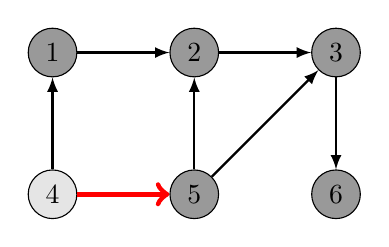
\begin{tikzpicture}[scale=0.9]
\node[draw, circle,fill=gray!80] (1) at (1,5) {$1$};
\node[draw, circle,fill=gray!80] (2) at (3,5) {$2$};
\node[draw, circle,fill=gray!80] (3) at (5,5) {$3$};
\node[draw, circle,fill=gray!20] (4) at (1,3) {$4$};
\node[draw, circle,fill=gray!80] (5) at (3,3) {$5$};
\node[draw, circle,fill=gray!80] (6) at (5,3) {$6$};

\path[draw,thick,->,>=latex] (1) -- (2);
\path[draw,thick,->,>=latex] (2) -- (3);
\path[draw,thick,->,>=latex] (4) -- (1);
%\path[draw,thick,->,>=latex] (4) -- (5);
\path[draw,thick,->,>=latex] (5) -- (2);
\path[draw,thick,->,>=latex] (5) -- (3);
\path[draw,thick,->,>=latex] (3) -- (6);

\path[draw=red,thick,->,line width=2pt] (4) -- (5);
\end{tikzpicture}
\end{center}

Thus, the final list is $[6,3,2,1,5,4]$.
We have processed all nodes, so a topological sort has
been found.
The topological sort is the reverse list
$[4,5,1,2,3,6]$:

\begin{center}
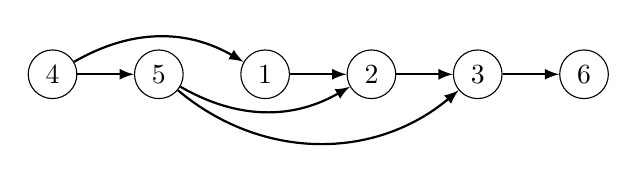
\begin{tikzpicture}[scale=0.9]
\node[draw, circle] (1) at (3,0) {$1$};
\node[draw, circle] (2) at (4.5,0) {$2$};
\node[draw, circle] (3) at (6,0) {$3$};
\node[draw, circle] (4) at (0,0) {$4$};
\node[draw, circle] (5) at (1.5,0) {$5$};
\node[draw, circle] (6) at (7.5,0) {$6$};

\path[draw,thick,->,>=latex] (1) -- (2);
\path[draw,thick,->,>=latex] (2) -- (3);
\path[draw,thick,->,>=latex] (4) edge [bend left=30] (1);
\path[draw,thick,->,>=latex] (4) -- (5);
\path[draw,thick,->,>=latex] (5) edge [bend right=30] (2);
\path[draw,thick,->,>=latex] (5) edge [bend right=40] (3);
\path[draw,thick,->,>=latex] (3) -- (6);
\end{tikzpicture}
\end{center}

Note that a topological sort is not unique,
but there can be several topological sorts for a graph.

\subsubsection{Example 2}

Let us now consider a graph for which we
cannot construct a topological sort,
because there is a cycle in the graph:

\begin{center}
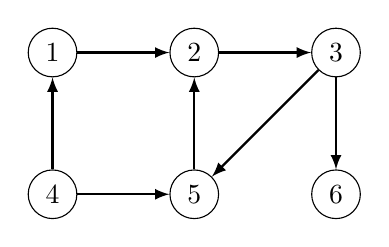
\begin{tikzpicture}[scale=0.9]
\node[draw, circle] (1) at (1,5) {$1$};
\node[draw, circle] (2) at (3,5) {$2$};
\node[draw, circle] (3) at (5,5) {$3$};
\node[draw, circle] (4) at (1,3) {$4$};
\node[draw, circle] (5) at (3,3) {$5$};
\node[draw, circle] (6) at (5,3) {$6$};

\path[draw,thick,->,>=latex] (1) -- (2);
\path[draw,thick,->,>=latex] (2) -- (3);
\path[draw,thick,->,>=latex] (4) -- (1);
\path[draw,thick,->,>=latex] (4) -- (5);
\path[draw,thick,->,>=latex] (5) -- (2);
\path[draw,thick,->,>=latex] (3) -- (5);
\path[draw,thick,->,>=latex] (3) -- (6);
\end{tikzpicture}
\end{center}
The search proceeds as follows:
\begin{center}
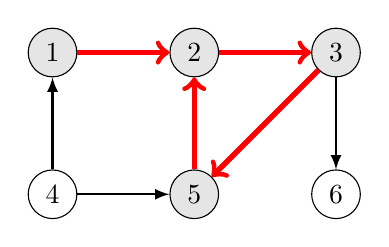
\begin{tikzpicture}[scale=0.9]
\node[draw, circle,fill=gray!20] (1) at (1,5) {$1$};
\node[draw, circle,fill=gray!20] (2) at (3,5) {$2$};
\node[draw, circle,fill=gray!20] (3) at (5,5) {$3$};
\node[draw, circle] (4) at (1,3) {$4$};
\node[draw, circle,fill=gray!20] (5) at (3,3) {$5$};
\node[draw, circle] (6) at (5,3) {$6$};

\path[draw,thick,->,>=latex] (4) -- (1);
\path[draw,thick,->,>=latex] (4) -- (5);
\path[draw,thick,->,>=latex] (3) -- (6);

\path[draw=red,thick,->,line width=2pt] (1) -- (2);
\path[draw=red,thick,->,line width=2pt] (2) -- (3);
\path[draw=red,thick,->,line width=2pt] (3) -- (5);
\path[draw=red,thick,->,line width=2pt] (5) -- (2);
\end{tikzpicture}
\end{center}
The search reaches node 2 whose state is 1,
which means the graph contains a cycle.
In this example, the cycle is $2 \rightarrow 3 \rightarrow 5 \rightarrow 2$.

\section{Dynamic programming}

If a directed graph is acyclic,
dynamic programming can be applied to it.
For example, we can efficiently solve the following
problems concerning paths from a starting node
to an ending node:

\begin{itemize}
\item how many different paths are there?
\item what is the shortest/longest path?
\item what is the minimum/maximum number of edges in a path?
\item which nodes certainly appear in any path?
\end{itemize}

\subsubsection{Counting the number of paths}

As an example, let us calculate the number of paths
from node 4 to node 6 in the following graph:

\begin{center}
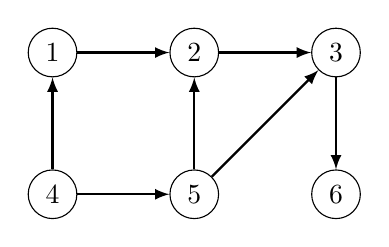
\begin{tikzpicture}[scale=0.9]
\node[draw, circle] (1) at (1,5) {$1$};
\node[draw, circle] (2) at (3,5) {$2$};
\node[draw, circle] (3) at (5,5) {$3$};
\node[draw, circle] (4) at (1,3) {$4$};
\node[draw, circle] (5) at (3,3) {$5$};
\node[draw, circle] (6) at (5,3) {$6$};

\path[draw,thick,->,>=latex] (1) -- (2);
\path[draw,thick,->,>=latex] (2) -- (3);
\path[draw,thick,->,>=latex] (4) -- (1);
\path[draw,thick,->,>=latex] (4) -- (5);
\path[draw,thick,->,>=latex] (5) -- (2);
\path[draw,thick,->,>=latex] (5) -- (3);
\path[draw,thick,->,>=latex] (3) -- (6);
\end{tikzpicture}
\end{center}

There are a total of three such paths:
\begin{itemize}
\item $4 \rightarrow 1 \rightarrow 2 \rightarrow 3 \rightarrow 6$
\item $4 \rightarrow 5 \rightarrow 2 \rightarrow 3 \rightarrow 6$
\item $4 \rightarrow 5 \rightarrow 3 \rightarrow 6$
\end{itemize}

To count the paths,
we go through the nodes in a topological sort,
and calculate for each node $x$ the number of paths
from node 4 to node $x$.
A topological sort for the above graph is as follows:
\begin{center}
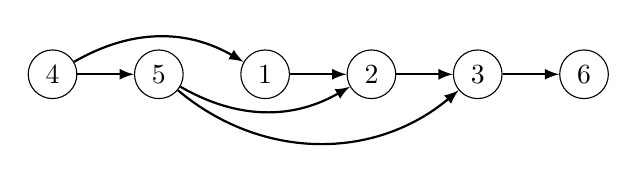
\begin{tikzpicture}[scale=0.9]
\node[draw, circle] (1) at (3,0) {$1$};
\node[draw, circle] (2) at (4.5,0) {$2$};
\node[draw, circle] (3) at (6,0) {$3$};
\node[draw, circle] (4) at (0,0) {$4$};
\node[draw, circle] (5) at (1.5,0) {$5$};
\node[draw, circle] (6) at (7.5,0) {$6$};

\path[draw,thick,->,>=latex] (1) -- (2);
\path[draw,thick,->,>=latex] (2) -- (3);
\path[draw,thick,->,>=latex] (4) edge [bend left=30] (1);
\path[draw,thick,->,>=latex] (4) -- (5);
\path[draw,thick,->,>=latex] (5) edge [bend right=30] (2);
\path[draw,thick,->,>=latex] (5) edge [bend right=40] (3);
\path[draw,thick,->,>=latex] (3) -- (6);
\end{tikzpicture}
\end{center}

Hence, the numbers of paths are as follows:
\begin{center}
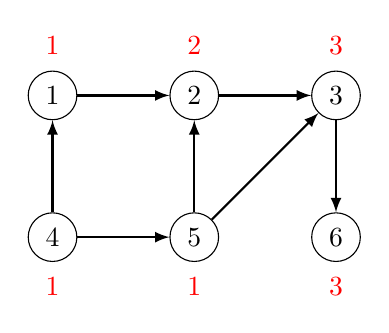
\begin{tikzpicture}[scale=0.9]
\node[draw, circle] (1) at (1,5) {$1$};
\node[draw, circle] (2) at (3,5) {$2$};
\node[draw, circle] (3) at (5,5) {$3$};
\node[draw, circle] (4) at (1,3) {$4$};
\node[draw, circle] (5) at (3,3) {$5$};
\node[draw, circle] (6) at (5,3) {$6$};

\path[draw,thick,->,>=latex] (1) -- (2);
\path[draw,thick,->,>=latex] (2) -- (3);
\path[draw,thick,->,>=latex] (4) -- (1);
\path[draw,thick,->,>=latex] (4) -- (5);
\path[draw,thick,->,>=latex] (5) -- (2);
\path[draw,thick,->,>=latex] (5) -- (3);
\path[draw,thick,->,>=latex] (3) -- (6);

\node[color=red] at (1,2.3) {$1$};
\node[color=red] at (3,2.3) {$1$};
\node[color=red] at (5,2.3) {$3$};
\node[color=red] at (1,5.7) {$1$};
\node[color=red] at (3,5.7) {$2$};
\node[color=red] at (5,5.7) {$3$};
\end{tikzpicture}
\end{center}

For example, since there are two paths
from node 4 to node 2 and
there is one path from node 4 to node 5,
we can conclude that there are three
paths from node 4 to node 3.

\subsubsection{Extending Dijkstra's algorithm}

\index{Dijkstra's algorithm}

A by-product of Dijkstra's algorithm is a directed, acyclic
graph that indicates for each node in the original graph
the possible ways to reach the node using a shortest path
from the starting node.
Dynamic programming can be applied to that graph.
For example, in the graph
\begin{center}
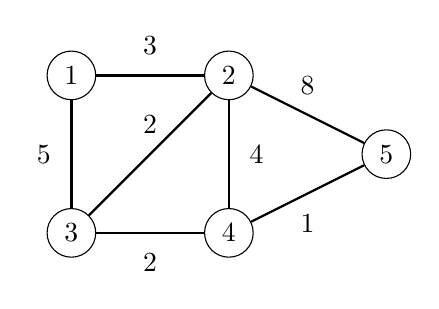
\begin{tikzpicture}
\node[draw, circle] (1) at (0,0) {$1$};
\node[draw, circle] (2) at (2,0) {$2$};
\node[draw, circle] (3) at (0,-2) {$3$};
\node[draw, circle] (4) at (2,-2) {$4$};
\node[draw, circle] (5) at (4,-1) {$5$};

\path[draw,thick,-] (1) -- node[font=\small,label=above:3] {} (2);
\path[draw,thick,-] (1) -- node[font=\small,label=left:5] {} (3);
\path[draw,thick,-] (2) -- node[font=\small,label=right:4] {} (4);
\path[draw,thick,-] (2) -- node[font=\small,label=above:8] {} (5);
\path[draw,thick,-] (3) -- node[font=\small,label=below:2] {} (4);
\path[draw,thick,-] (4) -- node[font=\small,label=below:1] {} (5);
\path[draw,thick,-] (2) -- node[font=\small,label=above:2] {} (3);
\end{tikzpicture}
\end{center}
the shortest paths from node 1 may use the following edges:
\begin{center}
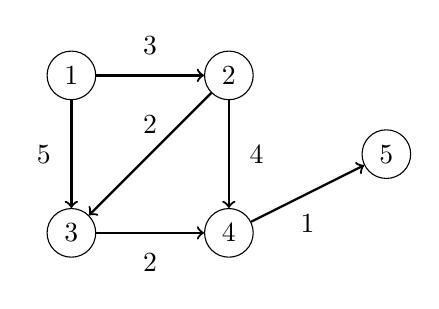
\begin{tikzpicture}
\node[draw, circle] (1) at (0,0) {$1$};
\node[draw, circle] (2) at (2,0) {$2$};
\node[draw, circle] (3) at (0,-2) {$3$};
\node[draw, circle] (4) at (2,-2) {$4$};
\node[draw, circle] (5) at (4,-1) {$5$};

\path[draw,thick,->] (1) -- node[font=\small,label=above:3] {} (2);
\path[draw,thick,->] (1) -- node[font=\small,label=left:5] {} (3);
\path[draw,thick,->] (2) -- node[font=\small,label=right:4] {} (4);
\path[draw,thick,->] (3) -- node[font=\small,label=below:2] {} (4);
\path[draw,thick,->] (4) -- node[font=\small,label=below:1] {} (5);
\path[draw,thick,->] (2) -- node[font=\small,label=above:2] {} (3);
\end{tikzpicture}
\end{center}

Now we can, for example, calculate the number of
shortest paths from node 1 to node 5
using dynamic programming:
\begin{center}
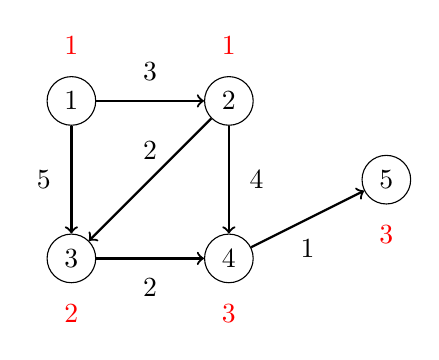
\begin{tikzpicture}
\node[draw, circle] (1) at (0,0) {$1$};
\node[draw, circle] (2) at (2,0) {$2$};
\node[draw, circle] (3) at (0,-2) {$3$};
\node[draw, circle] (4) at (2,-2) {$4$};
\node[draw, circle] (5) at (4,-1) {$5$};

\path[draw,thick,->] (1) -- node[font=\small,label=above:3] {} (2);
\path[draw,thick,->] (1) -- node[font=\small,label=left:5] {} (3);
\path[draw,thick,->] (2) -- node[font=\small,label=right:4] {} (4);
\path[draw,thick,->] (3) -- node[font=\small,label=below:2] {} (4);
\path[draw,thick,->] (4) -- node[font=\small,label=below:1] {} (5);
\path[draw,thick,->] (2) -- node[font=\small,label=above:2] {} (3);

\node[color=red] at (0,0.7) {$1$};
\node[color=red] at (2,0.7) {$1$};
\node[color=red] at (0,-2.7) {$2$};
\node[color=red] at (2,-2.7) {$3$};
\node[color=red] at (4,-1.7) {$3$};
\end{tikzpicture}
\end{center}

\subsubsection{Representing problems as graphs}

Actually, any dynamic programming problem
can be represented as a directed, acyclic graph.
In such a graph, each node corresponds to a dynamic programming state
and the edges indicate how the states depend on each other.

As an example, consider the problem
of forming a sum of money $x$
using coins
$\{c_1,c_2,\ldots,c_k\}$.
In this problem, we can construct a graph where
each node corresponds to a sum of money,
and the edges show how the coins can be chosen.
For example, for coins $\{1,3,4\}$ and $x=6$,
the graph is as follows:
\begin{center}
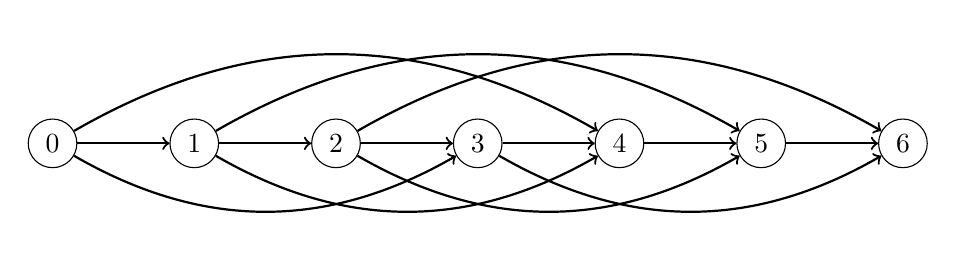
\begin{tikzpicture}[scale=0.9]
\node[draw, circle] (0) at (0,0) {$0$};
\node[draw, circle] (1) at (2,0) {$1$};
\node[draw, circle] (2) at (4,0) {$2$};
\node[draw, circle] (3) at (6,0) {$3$};
\node[draw, circle] (4) at (8,0) {$4$};
\node[draw, circle] (5) at (10,0) {$5$};
\node[draw, circle] (6) at (12,0) {$6$};

\path[draw,thick,->] (0) -- (1);
\path[draw,thick,->] (1) -- (2);
\path[draw,thick,->] (2) -- (3);
\path[draw,thick,->] (3) -- (4);
\path[draw,thick,->] (4) -- (5);
\path[draw,thick,->] (5) -- (6);

\path[draw,thick,->] (0) edge [bend right=30] (3);
\path[draw,thick,->] (1) edge [bend right=30] (4);
\path[draw,thick,->] (2) edge [bend right=30] (5);
\path[draw,thick,->] (3) edge [bend right=30] (6);

\path[draw,thick,->] (0) edge [bend left=30] (4);
\path[draw,thick,->] (1) edge [bend left=30] (5);
\path[draw,thick,->] (2) edge [bend left=30] (6);
\end{tikzpicture}
\end{center}

Using this representation,
the shortest path from node 0 to node $x$
corresponds to a solution with minimum number of coins,
and the total number of paths from node 0 to node $x$
equals the total number of solutions.

\section{Successor paths}

\index{successor graph}
\index{functional graph}

For the rest of the chapter,
we will concentrate on \key{successor graphs}
where the outdegree of each node is 1, i.e.,
exactly one edge starts at each node.
A successor graph consists of one or more
components, each of which contains
one cycle and some paths that lead to it.

Successor graphs are sometimes called
\key{functional graphs}.
The reason for this is that any successor graph
corresponds to a function $f$ that defines
the edges in the graph.
The parameter for the function is a node in the graph,
and the function gives the successor of the node.

\begin{samepage}
For example, the function
\begin{center}
\begin{tabular}{r|rrrrrrrrr}
$x$ & 1 & 2 & 3 & 4 & 5 & 6 & 7 & 8 & 9 \\
\hline
$f(x)$ & 3 & 5 & 7 & 6 & 2 & 2 & 1 & 6 & 3 \\
\end{tabular}
\end{center}
\end{samepage}
defines the following graph:
\begin{center}
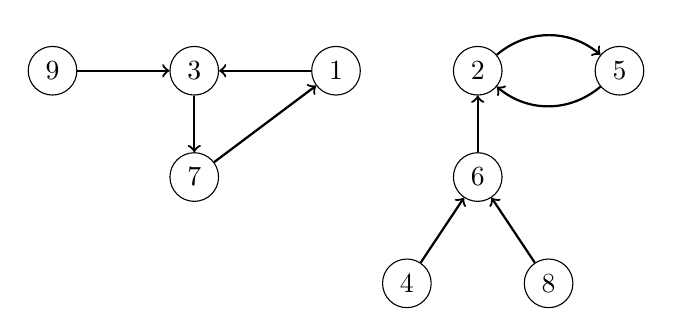
\begin{tikzpicture}[scale=0.9]
\node[draw, circle] (1) at (0,0) {$1$};
\node[draw, circle] (2) at (2,0) {$2$};
\node[draw, circle] (3) at (-2,0) {$3$};
\node[draw, circle] (4) at (1,-3) {$4$};
\node[draw, circle] (5) at (4,0) {$5$};
\node[draw, circle] (6) at (2,-1.5) {$6$};
\node[draw, circle] (7) at (-2,-1.5) {$7$};
\node[draw, circle] (8) at (3,-3) {$8$};
\node[draw, circle] (9) at (-4,0) {$9$};

\path[draw,thick,->] (1) -- (3);
\path[draw,thick,->] (2)  edge [bend left=40] (5);
\path[draw,thick,->] (3) -- (7);
\path[draw,thick,->] (4) -- (6);
\path[draw,thick,->] (5)  edge [bend left=40] (2);
\path[draw,thick,->] (6) -- (2);
\path[draw,thick,->] (7) -- (1);
\path[draw,thick,->] (8) -- (6);
\path[draw,thick,->] (9) -- (3);
\end{tikzpicture}
\end{center}

Since each node in a successor graph has a
unique successor, we can define a function $f(x,k)$
that returns the node that we will reach if
we begin at node $x$ and walk $k$ steps forward.
For example, in the above graph $f(4,6)=2$,
because we will reach node 2 by walking 6 steps from node 4:

\begin{center}
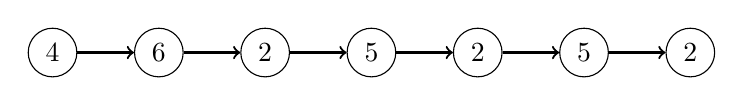
\begin{tikzpicture}[scale=0.9]
\node[draw, circle] (1) at (0,0) {$4$};
\node[draw, circle] (2) at (1.5,0) {$6$};
\node[draw, circle] (3) at (3,0) {$2$};
\node[draw, circle] (4) at (4.5,0) {$5$};
\node[draw, circle] (5) at (6,0) {$2$};
\node[draw, circle] (6) at (7.5,0) {$5$};
\node[draw, circle] (7) at (9,0) {$2$};

\path[draw,thick,->] (1) -- (2);
\path[draw,thick,->] (2) -- (3);
\path[draw,thick,->] (3) -- (4);
\path[draw,thick,->] (4) -- (5);
\path[draw,thick,->] (5) -- (6);
\path[draw,thick,->] (6) -- (7);
\end{tikzpicture}
\end{center}

A straightforward way to calculate a value of $f(x,k)$
is to start at node $x$ and walk $k$ steps forward, which takes $O(k)$ time.
However, using preprocessing, any value of $f(x,k)$
can be calculated in only $O(\log k)$ time.

The idea is to precalculate all values $f(x,k)$ where
$k$ is a power of two and at most $u$, where $u$ is
the maximum number of steps we will ever walk.
This can be efficiently done, because
we can use the following recursion:

\begin{equation*}
    f(x,k) = \begin{cases}
               f(x)              & k = 1\\
               f(f(x,k/2),k/2)   & k > 1\\
           \end{cases}
\end{equation*}

Precalculating values $f(x,k)$ takes $O(n \log u)$ time,
because $O(\log u)$ values are calculated for each node.
In the above graph, the first values are as follows:

\begin{center}
\begin{tabular}{r|rrrrrrrrr}
$x$ & 1 & 2 & 3 & 4 & 5 & 6 & 7 & 8 & 9 \\
\hline
$f(x,1)$ & 3 & 5 & 7 & 6 & 2 & 2 & 1 & 6 & 3 \\
$f(x,2)$ & 7 & 2 & 1 & 2 & 5 & 5 & 3 & 2 & 7 \\
$f(x,4)$ & 3 & 2 & 7 & 2 & 5 & 5 & 1 & 2 & 3 \\
$f(x,8)$ & 7 & 2 & 1 & 2 & 5 & 5 & 3 & 2 & 7 \\
$\cdots$ \\
\end{tabular}
\end{center}

After this, any value of $f(x,k)$ can be calculated
by presenting the number of steps $k$ as a sum of powers of two.
For example, if we want to calculate the value of $f(x,11)$,
we first form the representation $11=8+2+1$.
Using that,
\[f(x,11)=f(f(f(x,8),2),1).\]
For example, in the previous graph
\[f(4,11)=f(f(f(4,8),2),1)=5.\]

Such a representation always consists of
$O(\log k)$ parts, so calculating a value of $f(x,k)$
takes $O(\log k)$ time.

\section{Cycle detection}

\index{cycle}
\index{cycle detection}

Consider a successor graph that only contains
a path that ends in a cycle.
There are two interesting questions:
if we begin our walk at the starting node,
what is the first node in the cycle
and how many nodes does the cycle contain?

For example, in the graph

\begin{center}
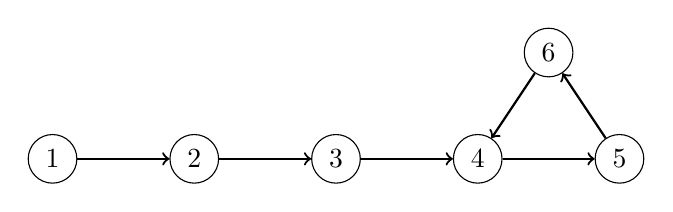
\begin{tikzpicture}[scale=0.9]
\node[draw, circle] (5) at (0,0) {$5$};
\node[draw, circle] (4) at (-2,0) {$4$};
\node[draw, circle] (6) at (-1,1.5) {$6$};
\node[draw, circle] (3) at (-4,0) {$3$};
\node[draw, circle] (2) at (-6,0) {$2$};
\node[draw, circle] (1) at (-8,0) {$1$};

\path[draw,thick,->] (1) -- (2);
\path[draw,thick,->] (2) -- (3);
\path[draw,thick,->] (3) -- (4);
\path[draw,thick,->] (4) -- (5);
\path[draw,thick,->] (5) -- (6);
\path[draw,thick,->] (6) -- (4);
\end{tikzpicture}
\end{center}
we begin our walk at node 1,
the first node that belongs to the cycle is node 4, and the cycle consists
of three nodes (4, 5 and 6).

An easy way to detect the cycle is to walk in the
graph and keep track of
all nodes that have been visited. Once a node is visited
for the second time, we can conclude
that the node is the first node in the cycle.
This method works in $O(n)$ time and also uses
$O(n)$ memory.

However, there are better algorithms for cycle detection.
The time complexity of such algorithms is still $O(n)$,
but they only use $O(1)$ memory.
This is an important improvement if $n$ is large.
Next we will discuss Floyd's algorithm that
achieves these properties.

\subsubsection{Floyd's algorithm}

\index{Floyd's algorithm}

\key{Floyd's algorithm} walks forward 
in the graph using two pointers $a$ and $b$.
Both pointers begin at a node $x$ that
is the starting node of the graph.
Then, on each turn, the pointer $a$ walks
one step forward and the pointer $b$
walks two steps forward.
The process continues until
the pointers meet each other:

\begin{lstlisting}
a = f(x);
b = f(f(x));
while (a != b) {
    a = f(a);
    b = f(f(b));
}
\end{lstlisting}

At this point, the pointer $a$ has walked $k$ steps
and the pointer $b$ has walked $2k$ steps,
so the length of the cycle divides $k$.
Thus, the first node that belongs to the cycle
can be found by moving the pointer $a$ to node $x$
and advancing the pointers
step by step until they meet again:

\begin{lstlisting}
a = x;
while (a != b) {
    a = f(a);
    b = f(b);
}
\end{lstlisting}

Now $a$ and $b$ point to the first node in the cycle
that can be reached from node $x$.
Finally, the length $c$ of the cycle
can be calculated as follows:

\begin{lstlisting}
b = f(a);
c = 1;
while (a != b) {
    b = f(b);
    c++;
}
\end{lstlisting}